\documentclass{beamer}
\usetheme{moloch}
\usepackage{lmodern} %czconki w rozmiarze 12
%\usepackage[latin2]{inputenc}
%\usepackage[T1]{fontenc}
%\usepackage[polish]{babel}
\usepackage{polski}
\usepackage{graphicx}
\usepackage{setspace}
\title{Gnuplot}

\begin{document}
\maketitle
\begin{frame}{Gnuplot}
    \begin{itemize}
        \item Narzędzie do:
        \begin{itemize}
            \item tworzenia grafiki,
            \item \emph{podstawowej} analizy danych.
        \end{itemize}
        \item Praca w trybie tekstowym
        \begin{itemize}
            \item interaktywnym,
            \item skryptowym.
        \end{itemize}
    \end{itemize}
\end{frame}
\begin{frame}[containsverbatim]{Podstawowe polecenia}
\begin{itemize}
    \item \begin{verbatim}
        plot ... 
    \end{verbatim}
    \item \verb|set|
    \begin{itemize}
        \item \verb|title|
        \item \verb|xlabel, ylabel|
        \item \verb|xrange, yrange|
        \item \verb|(x)yticks, (mx)myticks,...|
        \item \verb|grid|
    \end{itemize}
\end{itemize}
    
\end{frame}
\begin{frame}{Style linii}
\begin{figure}
    \centering
    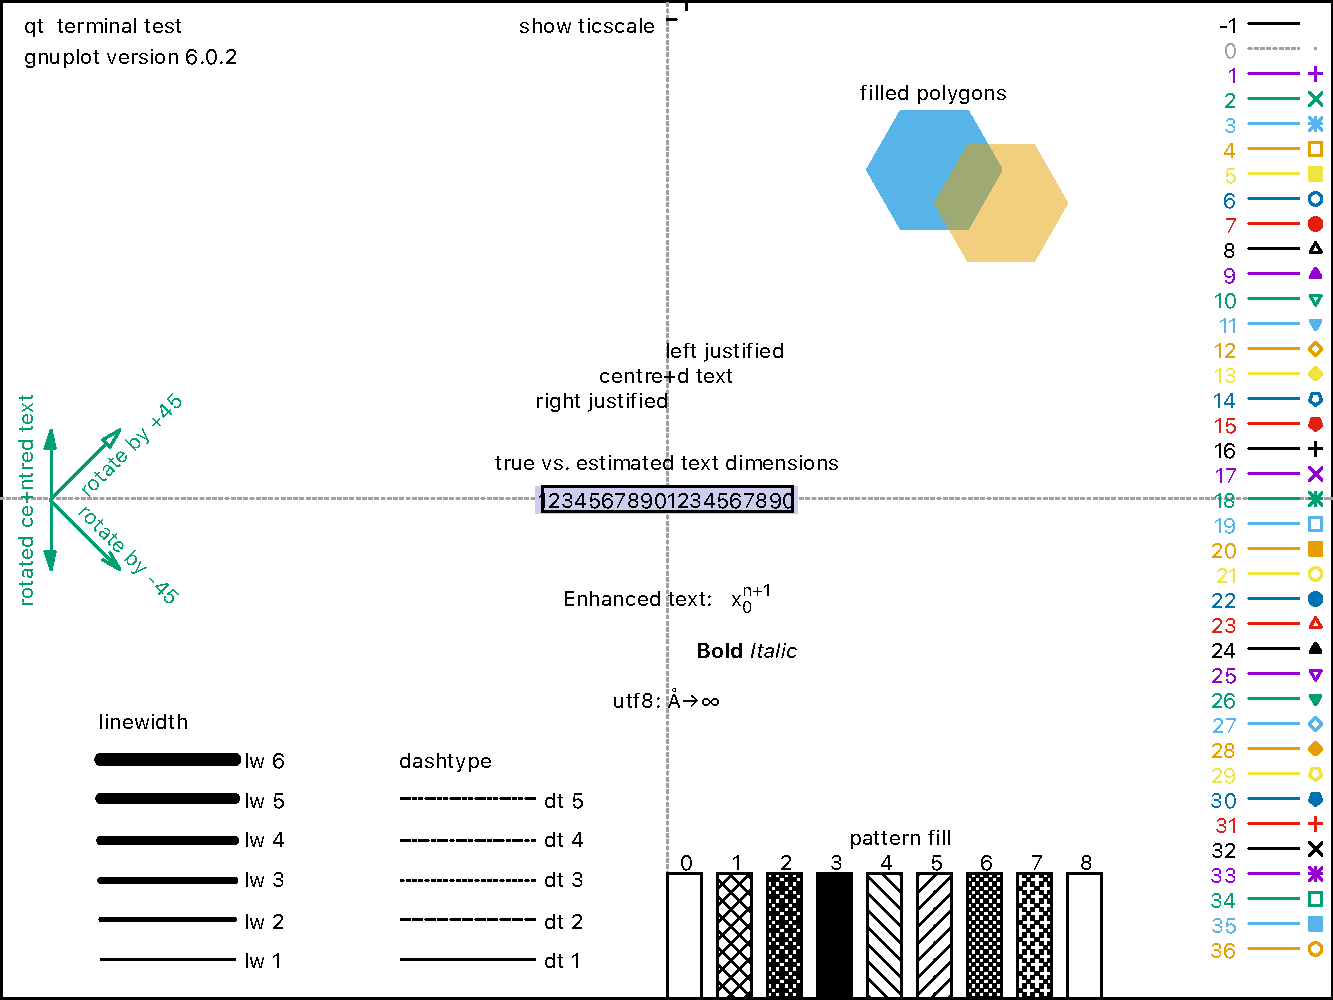
\includegraphics[width=0.7\linewidth]{test}
    \caption{Style linii}
    \label{fig:style_linii}
\end{figure}
    
\end{frame}

\begin{frame}[containsverbatim]{Style linii - c.d.}
\begin{itemize}
    \item \verb|plot sin(x) linetype 2, cos(x) linetype 4|
    \item \verb|plot sin(x) lt 2, cos(x) with points lt 4| \\[10pt]
    \item \verb|set linetype 6|
    \item  \verb|set linetype 6 dashtype 4|
\end{itemize}
\end{frame}

\begin{frame}[containsverbatim]{Dane}

\begin{itemize}
    \item \verb|plot "dane1.dat" using 1:2|
    \item \verb|plot "dane1.dat" using 1:($2**2)|
    \item \verb|plot ... w xyerrorbars|
    \item  \verb|plot "dane1.dat" smooth csplines|
\end{itemize}
    
\end{frame}
\begin{frame}{Frame Title}
    
\end{frame}

\begin{frame}[containsverbatim]{Niepewności pomiarowe w danych}
Przykład danych:

\begin{verbatim}
    #x y dx dy
    0.0  1.64 1.0 1.0
    1.0  1.27 1.0 1.0
    2.0  3.07 1.0 1.0
    3.0  2.53 1.0 1.0
    4.0  4.15 1.0 1.0
    10.0 5.11 1.0 5.0
\end{verbatim}
\end{frame}
\begin{frame}[containsverbatim]{\texttt{xyerrorbars}}
\setstretch{1.5}
    \begin{itemize}
        \item \verb|plot ... using 1:2:3 with xerrorbars|
        \item \verb|plot ... using 1:2:4 with yerrorbars|
        \item \verb|plot ... (using 1:2:3:4) with xyerrorbars|
    \end{itemize}
\end{frame}

    
\begin{frame}[containsverbatim]{Dopasowywanie funkcji}

\verb|f(x) = a*x + b|\\
\verb|g(x) = a*x**(1/2) + b|\\[2mm]
\verb|fit f(x) "dane1.dat" via a,b|

\end{frame}


% \section{Dopasowanie funkcji}

\frame{{Dopasowywanie funkcji}

Załóżmy, że mamy zbiór danych $\{ (x_i,y_i,\varepsilon_i )\} $, $ i = 1,...,N$, gdzie $\varepsilon_i$ jest niepewnością
wartości $y_i$, oraz funkcja $f(x;a_1,...,a_k)$. \\ 
Celem polecenia {\bf fit} jest minimalizacja
$$
\chi^2(\overline{a})=\sum_{i=1}^N \left[ \frac{y_i-f(x_i;\overline{a})}{\varepsilon_i} \right]^2
$$
względem $\overline{a} = a_1,...,a_k$.
}

\begin{frame}[containsverbatim]{Wizualizacja dopasowania}
    \verb|plot "" w xyerrorbars, g(x)|
\end{frame}

\begin{frame}[containsverbatim]{Aproksymacja krzywymi sklejanymi}
        \begin{itemize}
        \item \verb|plot ... smooth csplines|
        \item \verb|plot ... using 1:2:(1/$3**2) smooth acsplines|
    \end{itemize}
\end{frame}
\begin{frame}[containsverbatim]{Pliki wsadowe}
    \begin{itemize}
        \item \verb|gnuplot -c skrypt1.gp ARG1 ARG2 ARG3 ...|
    \end{itemize}
    \begin{verbatim}
        set title ARG1
        plot ARG2 with lines title "Wykres z pliku ".ARG2
        pause -1
    \end{verbatim}
\end{frame}
\begin{frame}[containsverbatim]{\texttt{Splot}}
\texttt{splot x**2+y**2}
\end{frame}
\begin{frame}{Wykresy parametryczne}
    \begin{itemize}
        \item \texttt{set param}
        \item zmienną staje się $t$ 
        \begin{itemize}
            \item (lub $(u,v)$),
        \end{itemize}
        \item podajemy $(x(t), y(t))$
        \begin{itemize}
            \item (lub $(x(u,v), y(u,v), z(u,v)$).
        \end{itemize}
    \end{itemize}
\end{frame}
\begin{frame}[containsverbatim]{Torus}
    \begin{verbatim}
        set urange [0:2*pi]
        set vrange [0:2*pi]
        splot (1+0.2*cos(v))*cos(u),\
            (1+0.2*cos(v))*sin(u),0.2*sin(v)
    \end{verbatim}
\end{frame}
\begin{frame}{Współrzędne biegunowe}
   \begin{itemize}
       \item \texttt{set polar}
       \item zmienną jest $t$ (kąt),
       \item podajemy $r(t).$
   \end{itemize}
\end{frame}
\begin{frame}[containsverbatim]{Histogramy}
\begin{verbatim}
    set data style histograms
    set key autotitle columnhead
    plot "przedmioty.dat" 
    using 2:xtic(1), ...
\end{verbatim}
\end{frame}
\begin{frame}[containsverbatim]{Wykresy pudełkowe}

    \begin{verbatim}
        set data style boxplot
        set style boxplot fraction 0.95
        plot "energia.dat" using (1.0):8:(0):4
    \end{verbatim}

\end{frame}
\end{document}